分层数据并行内核提供了实验性的替代语法,可以用工作组和工作项来表示内核,其中层次结构的每一层都使用parallel\_for嵌套调用。这种自顶向下的编程风格类似于编写并行循环,可能比其他两种内核形式使用的自底向上编程风格更为开发者和读者熟悉。\par

分层内核的复杂性在于,paralle\_for的嵌套调用会创建单独的SPMD环境,每个范围定义了新的“程序”,其应由与该范围相关的并行工作项执行。这种复杂性要求编译器进行分析,并可能使生成某些设备的代码复杂化。一些平台上用于分层并行内核的编译器技术仍然不成熟,性能与编译器实现的质量密切相关。\par

由于分层数据并行内核和为特定设备生成的代码之间的关系依赖于编译器,因此分层内核应该比显式的ND-Range内核更具描述性的结构。由于分层内核保留了控制任务映射工作项和工作组的能力,因此比基本内核更具有特定性。\par

\hspace*{\fill} \par %插入空行
\textbf{理解分层的数据并行内核}

分层数据并行内核的底层执行模型,与显式ND-Range数据并行内核的执行模型相同。工作项、子工作组和工作组具有相同的语义和执行保证。\par

然而,分层内核的不同作用域由编译器映射到不同的执行资源:外部作用域对每个工作组执行一次(就像由单个工作项执行一样),而内部作用域由工作组中的工作项并行执行。不同的作用域还控制内存中分配变量的位置,并且作用域的打开和关闭意味着启用工作组栅栏(以强制执行内存一致性)。\par

尽管工作组中的工作项仍然划分为子工作组,但不能在分层并行内核访问sub\_group类,将子工作组的概念合并到SYCL分层并行中,是比引入新类更重要的修改,这个工作正在进行中。\par

\hspace*{\fill} \par %插入空行
\textbf{编写分层的数据并行内核}

分层内核中,parallel\_for\_work\_group和parallel\_for\_work\_item可以取代parallel\_for,分别对应于工作组和工作项的并行性。parallel\_for\_work\_group作用域中的任何代码在工作组中只执行一次,并且在parallel\_for\_work\_group作用域中分配的变量对所有工作项都可见(在工作组本地内存中分配)。在parallel\_for\_work\_item范围内的任何代码,都是由工作组的工作项目并行执行,并且在parallel\_for\_work\_item范围内分配的变量对单个工作项都可见(可以分配在工作项的私有内存中)。\par

如图4-20所示,分层并行表示的内核与ND-Range内核非常相似。因此,应该把分层并行看作是一种生产力象征,不公开任何未通过ND-Range内核公开的功能,但可以提高代码的可读性和/或减少代码量。\par

\hspace*{\fill} \par %插入空行
图4-20 表示具有层次并行性的矩阵乘法
\begin{lstlisting}[caption={}]
range num_groups{N / B, N / B}; // N is a multiple of B
range group_size{B, B};
h.parallel_for_work_group(num_groups, group_size, [=](group<2> grp) {
	int jb = grp.get_id(0);
	int ib = grp.get_id(1);
	grp.parallel_for_work_item([&](h_item<2> it) {
		int j = jb * B + it.get_local_id(0);
		int i = ib * B + it.get_local_id(1);
		for (int k = 0; k < N; ++k)
		c[j][i] += a[j][k] * b[k][i];
	});
});
\end{lstlisting}

需要注意的是,传递给parallel\_for\_work\_group的范围指定了组的数量和可选组的大小,而不是像ND-Range parallel\_for那样指定了工作项的总数和工作组大小。内核函数可传入组类的实例,反映出范围与工作组的关系,而不与单个工作项相关系。\par

parallel\_for\_work\_item是group类的一个成员函数,只能在parallel\_for\_work\_group的作用域内调用。在其最简形式中,唯一的参数是接受h\_item类实例的函数,该函数可以执行的次数等于每个工作组请求的工作项的数量。parallel\_for\_work\_item的另一个特性是支持逻辑范围的能力,作为附加参数传递给函数。当指定一个逻辑范围时,每个物理工作项执行零个或多个函数实例,并且逻辑范围的逻辑项会轮询,并分配给物理工作项。\par

图4-21显示了由11个逻辑工作项组成的逻辑范围,和由8个物理工作项组成的底层物理范围间的映射示例。前三个工作项分配了功能的两个实例,而其他工作项只分配了一个。\par

\hspace*{\fill} \par %插入空行
图4-21 将大小为11的逻辑范围映射为大小为8的物理范围
\begin{center}
	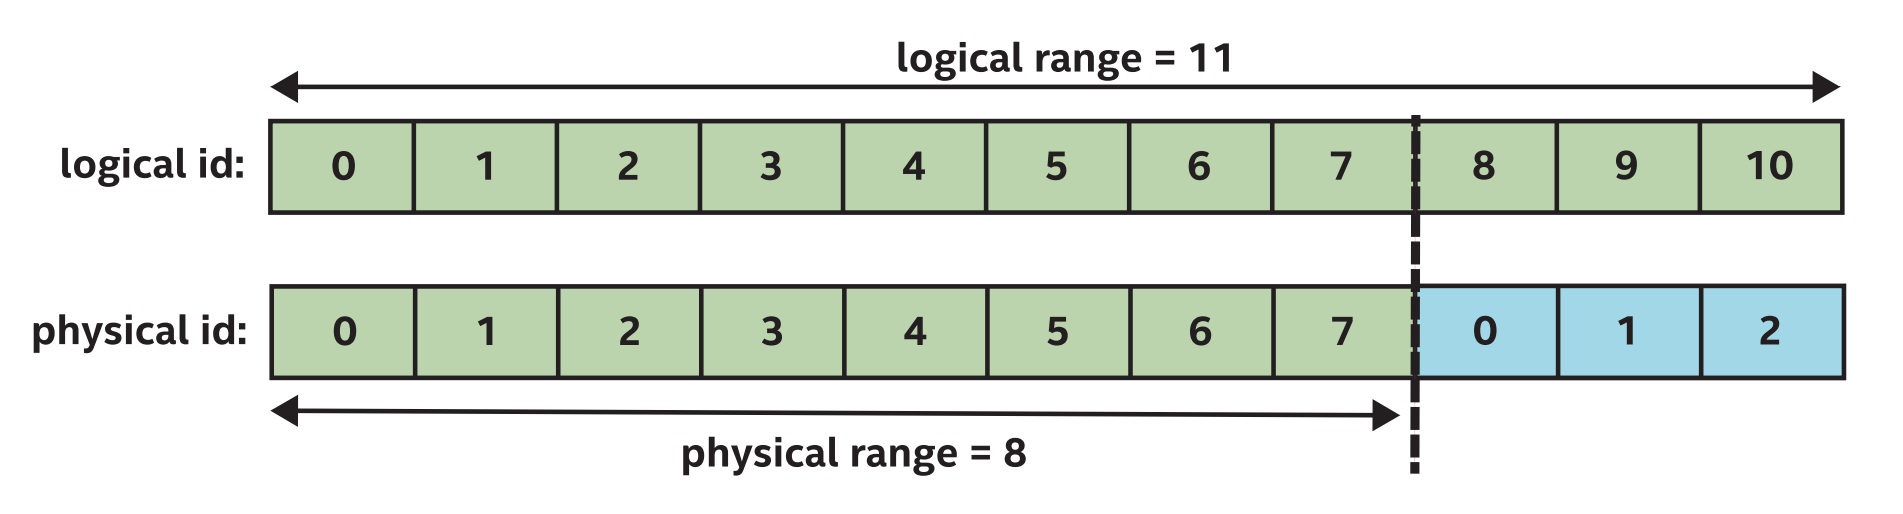
\includegraphics[width=1.\textwidth]{content/chapter-4/images/6}
\end{center}

如图4-22所示,将parallel\_for\_work\_group的可选组与parallel\_for\_work\_item的逻辑范围相结合,可以自由选择工作组大小,方便描述执行范围的能力。请注意,每个组执行的工作量与图4-20中相同,但是工作量已经与物理工作组大小不同了。\par

\hspace*{\fill} \par %插入空行
图4-22 用层次并行性和逻辑范围表示矩阵乘法
\begin{lstlisting}[caption={}]
range num_groups{N / B, N / B}; // N is a multiple of B
range group_size{B, B};
h.parallel_for_work_group(num_groups, [=](group<2> grp) {
	int jb = grp.get_id(0);
	int ib = grp.get_id(1);
	grp.parallel_for_work_item(group_size, [&](h_item<2> it) {
		int j = jb * B + it.get_logical_local_id(0);
		int i = ib * B + it.get_logical_local_id(1);
		for (int k = 0; k < N; ++k)
		c[j][i] += a[j][k] * b[k][i];
	});
});
\end{lstlisting}

\hspace*{\fill} \par %插入空行
\textbf{分层数据并行内核的细节}

分层数据并行内核重用来自ND-Range数据并行内核的group类,但需要将nd\_item替换为h\_item。引入新的私有内存类,以便在parallel\_for\_work\_group范围内对分配进行更严格的控制。\par

\hspace*{\fill} \par %插入空行
\textbf{h\_item类}

h\_item是item的变体,只能在parallel\_for\_work\_item作用域内使用。如图4-23,提供了一个类似的接口nd\_item:可以查询工作项的的工作组(get\_physical\_local\_id())或逻辑执行范围parallel\_for\_work\_item(使用get\_logical\_local\_id())。\par

\hspace*{\fill} \par %插入空行
图4-23 简化定义的h\_item类
\begin{lstlisting}[caption={}]
template <int Dimensions>
class h_item {
	public:
	// Return item's index in the kernel's execution range
	id<Dimensions> get_global_id() const;
	range<Dimensions> get_global_range() const;
	
	// Return the index in the work-group's execution range
	id<Dimensions> get_logical_local_id() const;
	range<Dimensions> get_logical_local_range() const;
	
	// Return the index in the logical execution range of the parallel_for
	id<Dimensions> get_physical_local_id() const;
	range<Dimensions> get_physical_local_range() const;
};
\end{lstlisting}

\hspace*{\fill} \par %插入空行
\textbf{private\_memory类}

private\_memory类提供了一种机制来声明每个工作项的私有变量,嵌套在同一个parallel\_for\_work\_group作用域内的多个parallel\_for\_work\_item都可以访问这些变量。\par

这个类非常必要,因为不同的分层并行性范围中的变量声明不同:如果编译器能够保证安全,则变量声明是私有的。我们不可能单独使用作用域,来表达变量是工作项私有的。\par

要了解为什么这是一个问题,回顾一下图4-22中的矩阵乘法内核。ib和jb变量是在parallel\_for\_work\_group作用域声明的,默认情况下应该在工作组的本地内存中分配!编译器很有可能不会犯这个错误,因为变量是只读的,可以在每个工作项上进行冗余计算,但语言并没有这样的保证。如果想确定一个变量是否在工作项私有内存中,需要将变量声明包装在private\_memory类的实例中,如图4-24所示。\par

\hspace*{\fill} \par %插入空行
图4-24 简化定义的private\_memory类
\begin{lstlisting}[caption={}]
template <typename T, int Dimensions = 1>
class private_memory {
	public:
	// Construct a private variable for each work-item in the group
	private_memory(const group<Dimensions>&);
	
	// Return the private variable associated with this work-item
	T& operator(const h_item<Dimensions>&);
};
\end{lstlisting}

例如,如果使用private\_memory类重写矩阵乘法内核,把变量定义为private\_memory<int> ib(grp),并且对这些变量的访问变成ib[item]。这样,使用private\_memory类的代码非常难读,而在parallel\_for\_work\_item范围中声明则会更简单。\par

如果工作项私有变量在多个parallel\_for\_work\_item范围内,并且在同一parallel\_for\_work\_group上使用,建议只使用private\_memory类,可以避免多余地计算。要不就依赖现代优化编译器的能力,并且只有在变量分析失败时才在parallel\_for\_work\_item范围声明变量(记住,也要向编译器供应商报告问题)。\par


















